\section{Previous Implementations of Secure Facial Recognition}

%% THIS SECTION IS MARKED FOR DELETION / AMPUTATION
% CryptoImg

% example of homomorphic encryption / image manipulation past work

% minor limitation: improvement on previous work, but not a direct comparison

% major limitation: does not discuss security: are modified images also secure?

%There has been work done regarding the application of homomorphic cryptosystems in image processing. In particular, Ziad, et al. introduced a library called \textit{CryptoImg} that uses the homomorphic properties of the Paillier cryptosystem to apply image operations securely \cite{ziad_cryptoimg:_2016}. This shows that it is indeed possible to do various image operations in a homomorphic cryptosystem. Ziad, et al. also showed experimental results establishing the slow performance of image operations uner a homomorphic cryptosystem. For instance, while sharpening and applying a Sobel filter each take less than a second when applied to a $512\times 512$ plaintext image, when applied to an encrypted image, sharpening required at least 238.257 seconds, and applying the Sobel filter required at least 147.567 seconds \cite{ziad_cryptoimg:_2016}.

%However, a major limitation of \textit{CryptoImg} is that it does not consider image security. Even though the authors have established that the Paillier cryptosystem itself cannot be broken \cite{ziad_cryptoimg:_2016}, we believe that a cryptanalysis of the encrypted images after they have been operated is necessary, since image operations may be considered additional information in a known plaintext attack.

%Furthermore, Ziad, et al. only presented a visual comparison and evaluation to establish the quality of the recovered images. We believe that additional image quality benchmarks, such as those presented in \cite{ahmed_benchmark_2016, ahmad_efficiency_2012}, would allow for quantitative comparisons of image quality.

%This study can be further improved by also considering the use of fully homomorphic cryptosystems such as the one presented by Dasgupta and Pal \cite{dasgupta_design_2016}, and the fully homomorphic cryptosystem introduced by Smart and Vercauteren \cite{hutchison_fully_2010} and improved by Gentry and Halevi  \cite{hutchison_implementing_2011}. These fully homomorphic cryptosystems have yet to be implemented for image processing operations.

% HElib
%Another related work would be the implementation of a fully homomorphic encryption. Halevi and Shoup \cite{garay_algorithms_2014} introduced \textit{HElib}, a library that implements the Brakerski--Gentry--Vaikuntanathan (BGV) homomorphic cryptosystem. This library also makes use of various optimizations to speed up the homomorphic operations, due to homomorphic cryptosystems being slower than other cryptosystems \cite{sen_homomorphic_2013}.

Erkin, et al. \cite{hutchison_privacy-preserving_2009-2} devised a method to incorporate the use of homomorphic cryptosystems into the eigenfaces method. In their study, they proposed a two-party system where Alice holds an encrypted image $\left[\Gamma\right]$, while Bob maintains a database of $K$ eigenfaces $\mathbf{u}_1, \ldots, \mathbf{u}_K$, and feature vectors $\Omega_1, \ldots, \Omega_M$ in the clear.

\begin{figure}[!h]
    \centering
    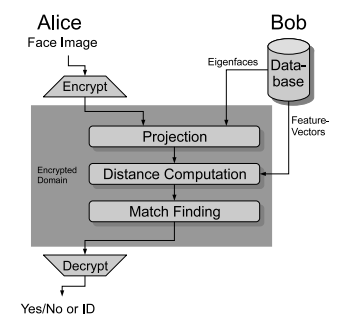
\includegraphics[width=7cm]{figures/secure_eigenfaces.png}
    \caption{Diagram of the privacy-preserving facial recognition process \cite{hutchison_privacy-preserving_2009-2}.}
\end{figure}


In order to ensure privacy, the steps in the eigenfaces algorithm, namely: projection, distance computation, and match finding, are done within the encrypted domain, i.e., using the operations in the Paillier cryptosystem.

Projection is similar to that of the original eigenfaces algorithm, except the operations are replaced with their respective operations in the cryptosystem. Distance computation in this version is somewhat different from the original eigenfaces method, in that it deals with the square of the Euclidean distance since the relative order of the distances is only important when comparing these during the match finding step \cite{hutchison_privacy-preserving_2009-2}.
\begin{align*}
    d_i &= \left\lVert \Omega_i - \bar{\Omega} \right\rVert ^2 = \sum_{j=1}^{K} \left(\omega_{ij} - \bar{\omega}_j\right)^2 \\
        &= \underbrace{\sum_{j=1}^{K} \omega_{ij}^2}_{\mathcal{S}_1} + \underbrace{\sum_{j=1}^{K} \left(-2 \omega_{ij} \bar{\omega_j}\right)}_{\mathcal{S}_2} + \underbrace{\sum_{j=1}^{K} \bar{\omega}_{j}^2}_{\mathcal{S}_3}
\end{align*}

Computing for the distances within Paillier would just be multiplying the encrypted sums together.
\[
\left[d_i\right] = \left[\mathcal{S}_1\right] \cdot \left[\mathcal{S}_2\right] \cdot \left[\mathcal{S}_3\right]
\]

The terms $\left[\mathcal{S}_1\right]$ and $\left[\mathcal{S}_2\right]$ can be easily computed by Bob, since he already knows both $\omega_i$ in the clear and $\left[\bar{\omega}_i\right]$ which is in encrypted form. Computing for $\left[\mathcal{S}_3\right]$ is trickier because Bob cannot compute for $\left[\bar{\omega}_i^2\right]$ because pairwise multiplication is not supported in Paillier, that is why Bob needs help from Alice to square a number through a protocol described below \cite{hutchison_privacy-preserving_2009-2}.

Before Bob sends $\left[\bar{\omega}_i\right]$ to Alice for squaring, he adds a random number $r_i$ to compute $\left[x_i\right] = \left[\bar{\omega}_i + r_i\right] = \left[\bar{\omega}_i\right] \cdot \left[r_i\right]$, where $r_i$ is obviously distinct for every $i$, then sends $\left[x_i\right]$ to Alice. She then decrypts it and computes $x_i^2$, and then computes $\mathcal{S}_3^\prime = \sum_{i=1}^{K} x_i^2$, after which she encrypts the sum and sends $\left[\mathcal{S}_3^\prime\right]$ to Bob. Now, he can compute for $\left[\mathcal{S}_3\right]$ as follows:
\[
\left[\mathcal{S}_3\right] = \left[\mathcal{S}_3^\prime\right] \cdot \prod_{j=1}^{K} \left(\left[\bar{\omega}_j\right]^{-2r_j} \cdot \left[-r_j^2\right]\right)
\]

The protocol for squaring a number as described earlier is a workaround for the limitations of Paillier or any other partially homomorphic cryptosystem that only supports addition and scalar multiplication. This can be possibly extended so that operations such as pairwise multiplication and exponentiation are also supported, provided that the protocol involves two parties.

The match finding step is done by comparing the distances obtained from the previous step to a specified threshold $T$. If the minimum distance is smaller than $T$, then a match is found, and the encrypted identity of the match is returned to Alice \cite{hutchison_privacy-preserving_2009-2}. Getting the minimum among the encrypted distances would involve comparing two encrypted numbers, which Paillier does not support. Instead, the DGK cryptosystem \cite{pieprzyk_efficient_2007} is used for the comparison protocol.
